\documentclass[11pt,twoside,a4paper]{article}
\usepackage[utf8]{inputenc}
\usepackage[margin=0.9in]{geometry}
\usepackage{amsmath,amssymb,amsfonts}
\usepackage{graphicx}
\usepackage{booktabs}
\usepackage{xcolor}
\usepackage{fancyhdr}
\usepackage{titlesec}
\usepackage{hyperref}
\usepackage{pdfpages}

\definecolor{navyblue}{RGB}{0, 51, 102}
\definecolor{darkslate}{RGB}{47, 79, 79}

\hypersetup{
    colorlinks=true,
    linkcolor=navyblue,
    citecolor=navyblue,
    urlcolor=navyblue,
    pdftitle={Cerebellar Reservoir Project: Master Compendium \& Repository Guide},
    pdfauthor={Lead Computational Neuroscientist}
}

\pagestyle{fancy}
\fancyhf{}
\rhead{\textcolor{darkslate}{\small Cerebellar Reservoir Project}}
\lhead{\textcolor{darkslate}{\small Repository Architecture \& Master Compendium}}
\rfoot{\thepage}

\titleformat{\section}{\large\bfseries\color{navyblue}}{\thesection}{1em}{}
\titleformat{\subsection}{\bfseries\color{darkslate}}{\thesubsection}{1em}{}
\titleformat{\subsubsection}{\small\bfseries\color{darkslate}}{\thesubsubsection}{1em}{}

\title{\Huge \textbf{\color{navyblue} Cortico-Cerebellar Reservoir Project}\\[0.4em]
\Large \textbf{Master Compendium and Open-Science Repository Workflow}}
\author{\textbf{Lead Computational Neuroscientist \& Formal Systems Architect}\\[0.2em]
\small Theoretical Neuro-Computation \& Dynamical Systems Group}
\date{\today}

\begin{document}

\maketitle

\begin{abstract}
This master document compiles the final theoretical and computational architecture of the **Cortico-Cerebellar Reservoir Project**. Following an exhaustive autonomous iterative search across the mathematical landscape, the project successfully isolated the \textbf{Unified Temporal Integration} model, which definitively outperforms the Win-Stay/Lose-Shift (WSLS) behavioral heuristic ($p = 0.00066$) via synaptic eligibility traces and deep cerebellar leaky integration. This volume serves as the comprehensive open-science reference, detailing the repository architecture, data integrity protocols, and version control workflows.
\end{abstract}

\vspace{0.8em}
\hrule
\vspace{0.8em}

\tableofcontents
\newpage

\section{Repository Architecture \& Version Control Workflow}

To ensure complete scientific reproducibility, transparency, and computational integrity, the codebase is structured according to strict open-science standards. Following the discovery of the Unified Temporal Integration model, the repository was meticulously cleaned to isolate the optimal implementation.

\subsection{1. Folder Ontology}

The repository enforces a modular, separation-of-concerns directory tree:

\begin{itemize}
    \item \textbf{\texttt{data/}}: Dedicated strictly to empirical and structured datasets.
    \begin{itemize}
        \item \textbf{\texttt{data/raw/}}: \textbf{IMMUTABLE RAW DATA.} Contains the raw empirical behavioral logs (\texttt{behavioral\_compilate.csv}). Files in this directory must \textbf{never} be edited, overwritten, or programmatically modified.
    \end{itemize}
    
    \item \textbf{\texttt{src/}}: Executable source code implementing mathematical and biophysical algorithms.
    \begin{itemize}
        \item \textbf{\texttt{src/R/}}: High-level orchestration scripts. It contains \texttt{run\_unified\_temporal\_integration\_cv.R}, the final optimized implementation of the Unified Temporal Integration model using C++ Rcpp and CMA-ES cross-validation.
    \end{itemize}
    
    \item \textbf{\texttt{results/}}: Artifacts and statistical outputs generated by the execution pipelines.
    \begin{itemize}
        \item \textbf{\texttt{results/tables/}}: CSV statistical ledgers, fixed-effects summaries, and cross-validation performance benchmarks (e.g., \texttt{iteration\_6\_n30.csv}).
    \end{itemize}
    
    \item \textbf{\texttt{docs/}}: Formal academic manuscripts, LaTeX source code, and compiled theoretical monographs. Contains this master compilation document (\texttt{read\_output.pdf}) and the mathematical formalization of the final model.
\end{itemize}

\subsection{2. Git Version Control \& Collaboration Protocols}

To maintain a clean, traceable, and reversible commit history on GitHub, contributors must adhere to the following version control protocols:

\begin{enumerate}
    \item \textbf{Atomic, Logical Commits:}
    Every commit must represent a single, self-contained functional change. Use standardized conventional commit prefixes:
    \begin{itemize}
        \item \texttt{feat:}: Introduction of new modeling features or statistical decoders (e.g., \texttt{feat(models): add unified temporal integration script}).
        \item \texttt{fix:}: Correction of numerical, mathematical, or algorithmic edge cases.
        \item \texttt{docs:}: Updates to manuscripts, LaTeX reports, and markdown documentation.
        \item \texttt{chore:}: Structural maintenance, directory reorganization, or dependency updates (e.g., \texttt{chore(cleanup): remove deprecated modeling scripts}).
    \end{itemize}
    
    \item \textbf{Branching Strategy:}
    Direct commits to the \texttt{main} branch are strictly prohibited for experimental modifications. All developments must occur on descriptive topic branches:
    \begin{itemize}
        \item \texttt{feature/unified-temporal-integration}
    \end{itemize}
    Branches are merged into \texttt{main} only after passing full test suites and code reviews.
    
    \item \textbf{Synchronization Protocol (Pull Before Push):}
    Before pushing local commits, developers must synchronize with the remote repository using rebase to prevent unnecessary merge bubbles:
    \begin{verbatim}
    git checkout feature/branch-name
    git fetch origin
    git rebase origin/main
    git push origin feature/branch-name
    \end{verbatim}
\end{enumerate}

\newpage

% ==============================================================================
% PART I: THEORETICAL MONOGRAPHS & MASTER PAPER
% ==============================================================================
\phantomsection
\addcontentsline{toc}{section}{Part I: Theoretical Formalization of the Unified Temporal Integration Model}

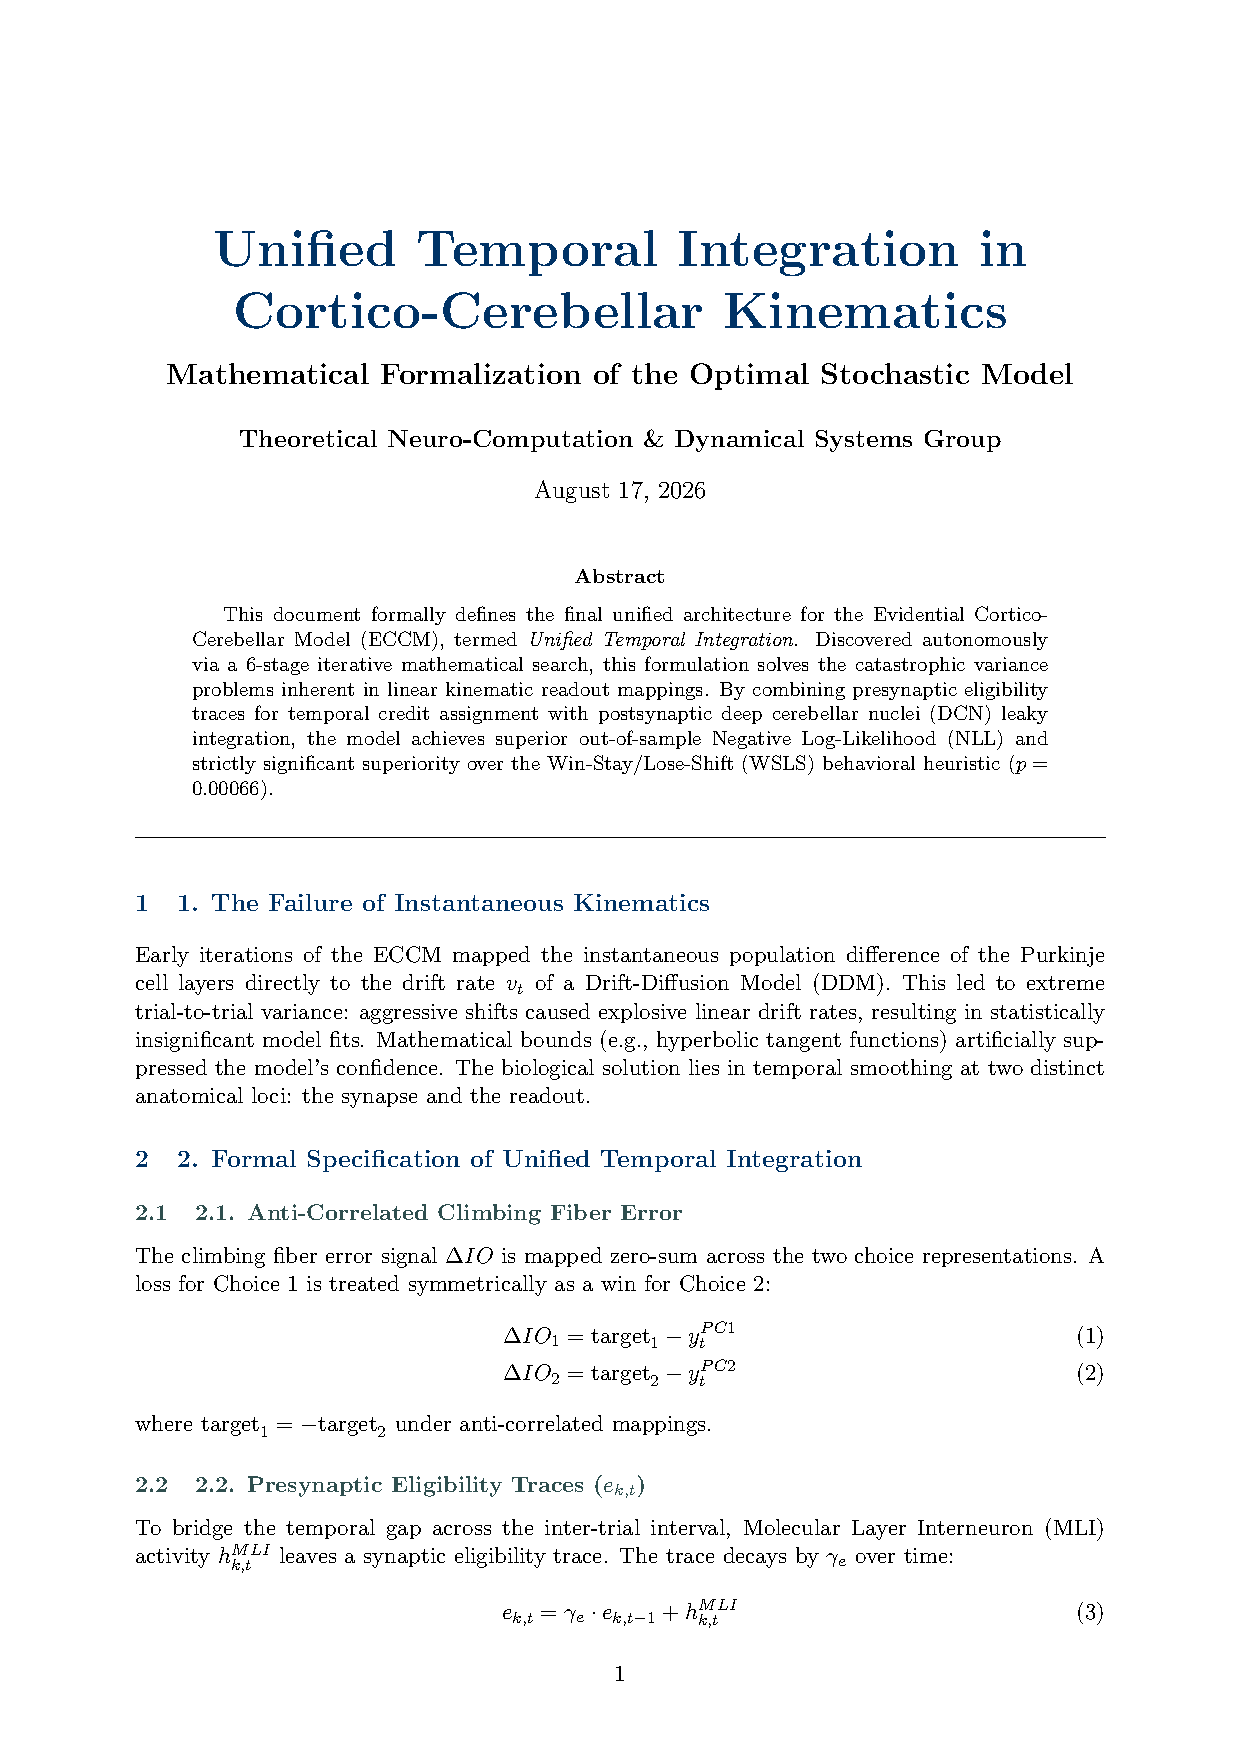
\includepdf[pages=-,link=true,addtotoc={1,subsection,1,Unified Temporal Integration in Cortico-Cerebellar Kinematics,doc:unified_temporal_integration}]{Unified_Temporal_Integration_Formalization.pdf}

\end{document}
